\chapter{Physics, Animations, and Relative Motion}
\label{chap:animations}

\section{Overview of Kinematic Systems}
A static 3D world fails to convey the vitality of a Japanese festival. \textit{Matsuri Nights} incorporates six interconnected kinematic and physics animation systems. These systems specifically demonstrate \textbf{motion relative to another object's reference frame}, hierarchical articulation, and continuous collision detection.

\section{System 1: Street Lantern Harmonic Pendulum Swing}
\subsection{Hierarchical Formulation}
Overhead street lanterns are assembled from two hierarchical nodes:
\begin{enumerate}
    \item \textbf{Parent Anchor Node (\texttt{ropePivot}):} Attached to the catenary suspension cable at $(x_{\text{span}}, y_{\text{cable}}, z_{\text{span}})$. Its local transformation contains zero translation but an oscillating $Z$-axis Euler rotation:
    \begin{equation}
    \theta_{\text{pivot}}(t) = \theta_0 \cdot \sin(\omega_{\text{swing}} t + \phi_k)
    \end{equation}
    where amplitude $\theta_0 = 12.0^\circ$, frequency $\omega_{\text{swing}} = 1.85\,\text{rad/s}$, and $\phi_k$ is a staggered phase offset.
    \item \textbf{Child Body Node (\texttt{lanternBody}):} Positioned at a negative vertical offset along local $Y$ ($y_{\text{local}} = -1.2\,\text{m}$). As the parent rotates, the child sweeps through a circular pendulum arc in world space:
    \begin{equation}
    \mathbf{p}_{\text{lantern}}(t) = \mathbf{M}_{\text{pivot}}(t) \cdot \begin{bmatrix} 0 \\ -1.2 \\ 0 \\ 1 \end{bmatrix}
    \end{equation}
\end{enumerate}

\subsection{Coupling to Dynamic Moving Lights}
Point Lights 3 and 4 query \texttt{lanternBody->getWorldPosition()} every frame (\texttt{src/Scene.h: lines 813--824}). Consequently, the illumination cast upon the cobblestone street and house facades swings in real time with the lanterns.

\section{System 2: Magic Orb Orbital Hierarchy}
\subsection{Nested Reference Frame Hierarchy}
The theatrical stage features an articulated magician figure performing with a glowing mystical orb. The orb is not animated in world coordinates; rather, it is anchored six levels deep within the magician's skeletal hierarchy:
\begin{equation}
\text{World} \to \text{Stage} \to \text{Magician Root} \to \text{Torso} \to \text{Right Shoulder} \to \text{Hand Bone} \to \text{Magic Orb}
\end{equation}
Relative to the moving hand bone coordinate frame, the orb executes harmonic elliptical orbital motion:
\begin{equation}
\begin{aligned}
x_{\text{local}}(t) &= R_{\text{orbit}} \cdot \cos(\omega_{\text{orb}} t) \\
z_{\text{local}}(t) &= R_{\text{orbit}} \cdot \sin(\omega_{\text{orb}} t) \\
y_{\text{local}}(t) &= y_0 + A_{\text{levitate}} \cdot \sin(2\omega_{\text{orb}} t)
\end{aligned}
\end{equation}
where $R_{\text{orbit}} = 0.45\,\text{m}$, $\omega_{\text{orb}} = 2.4\,\text{rad/s}$, and $A_{\text{levitate}} = 0.12\,\text{m}$.
Point Light 0 tracks the orb's world position, illuminating the magician's face, stage backdrop, and audience spectators with pulsing cyan radiance.

\begin{figure}[H]
\centering
\begin{subfigure}[b]{0.48\textwidth}
  \centering
  \IfFileExists{figures/ss_04_magic_show_orb.png}{%
    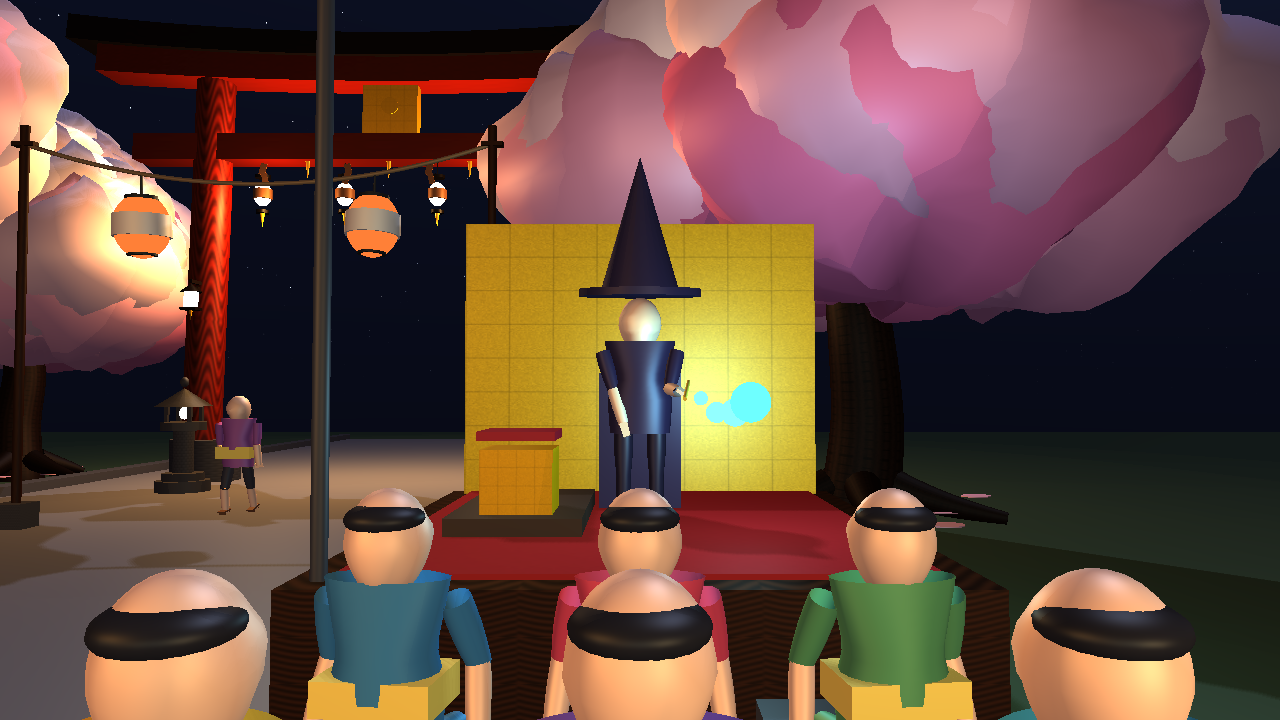
\includegraphics[width=\textwidth]{figures/ss_04_magic_show_orb.png}%
  }{\fbox{ss\_04}}
  \caption{Magician Figure with Orbiting Cyan Orb}
  \label{fig:magic_orb}
\end{subfigure}\hfill
\begin{subfigure}[b]{0.48\textwidth}
  \centering
  \IfFileExists{figures/ss_05_vanishing_box.png}{%
    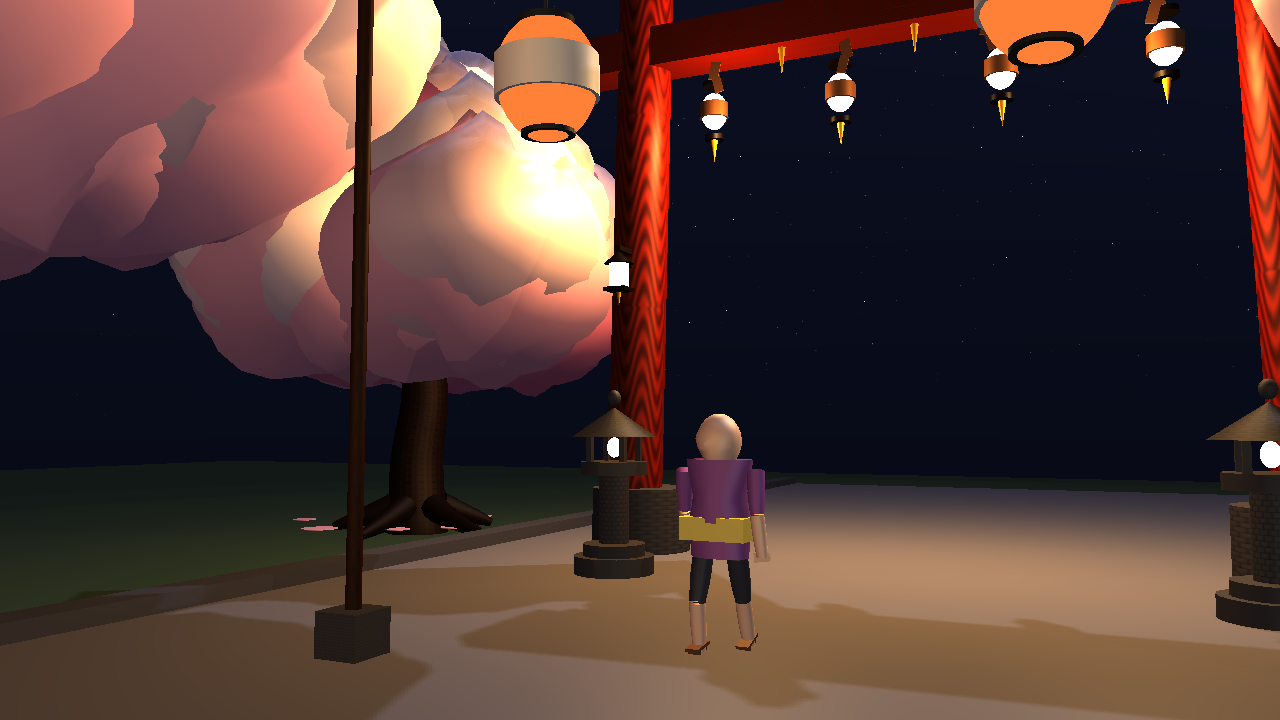
\includegraphics[width=\textwidth]{figures/ss_05_vanishing_box.png}%
  }{\fbox{ss\_05}}
  \caption{Vanishing Box Illusion Trick}
  \label{fig:vanishing_box}
\end{subfigure}
\caption{Theatrical Magic Show animations and hierarchical reference frames.}
\label{fig:magic_show_figures}
\end{figure}

\section{System 3: Takoyaki Projectile Hops and Kakigori Shaver Wheel}
\subsection{Takoyaki Food Stall Kinematics}
Each of the six individual octopus balls on the hot cast-iron griddle executes continuous jumping motion. Using Equation~\ref{eq:takoyaki_projectile}, vertical displacement follows a parabolic trajectory ($h_{\text{max}} = 0.18\,\text{m}$, $T = 0.95\,\text{s}$) while rotating continuously about the $Y$-axis ($360^\circ/\text{s}$).

\subsection{Kakigori Shaved Ice Machine Kinematics}
The vintage shaved ice machine features an iron flywheel crank rotating at $\omega_{\text{flywheel}} = 3.6\,\text{rad/s}$, geared to an internal ice block blade. On the counter, six colorful shaved ice bowls rotate synchronously.

\begin{figure}[H]
\centering
\begin{subfigure}[b]{0.48\textwidth}
  \centering
  \IfFileExists{figures/ss_06_takoyaki_stall.png}{%
    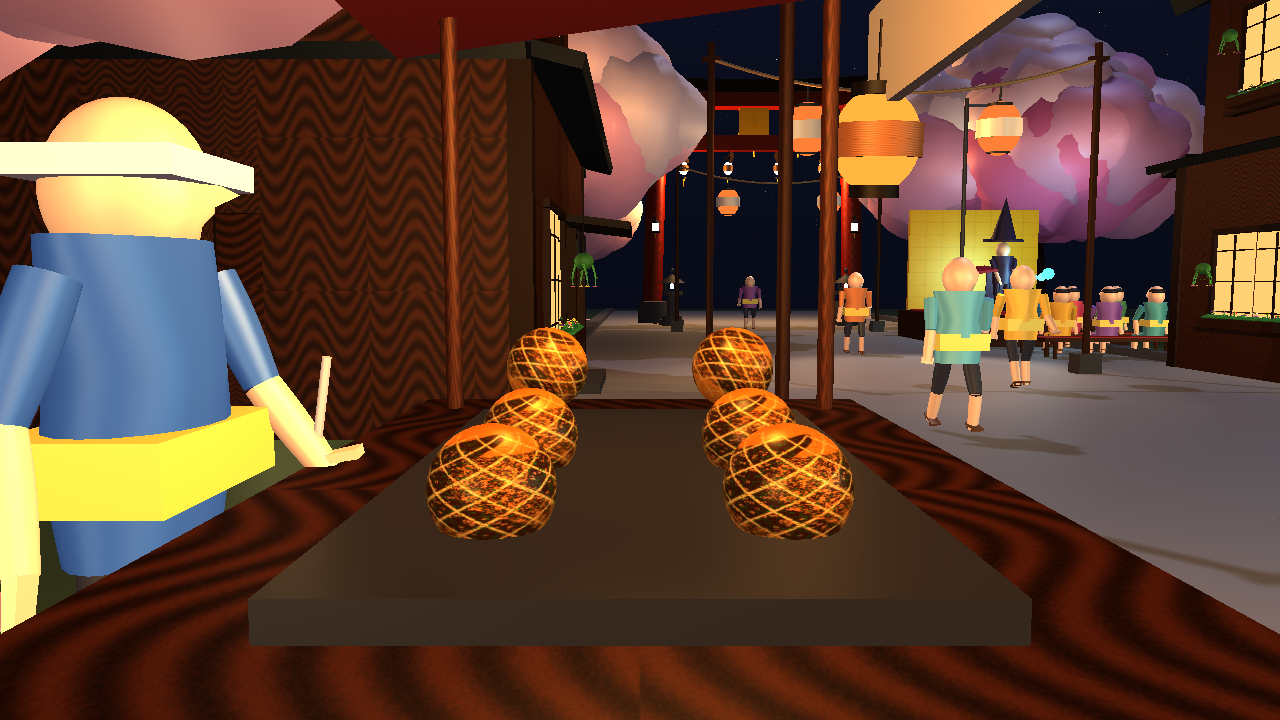
\includegraphics[width=\textwidth]{figures/ss_06_takoyaki_stall.png}%
  }{\fbox{ss\_06}}
  \caption{Takoyaki Food Stall with Hopping Balls}
  \label{fig:takoyaki_stall}
\end{subfigure}\hfill
\begin{subfigure}[b]{0.48\textwidth}
  \centering
  \IfFileExists{figures/ss_07_kakigori_stall.png}{%
    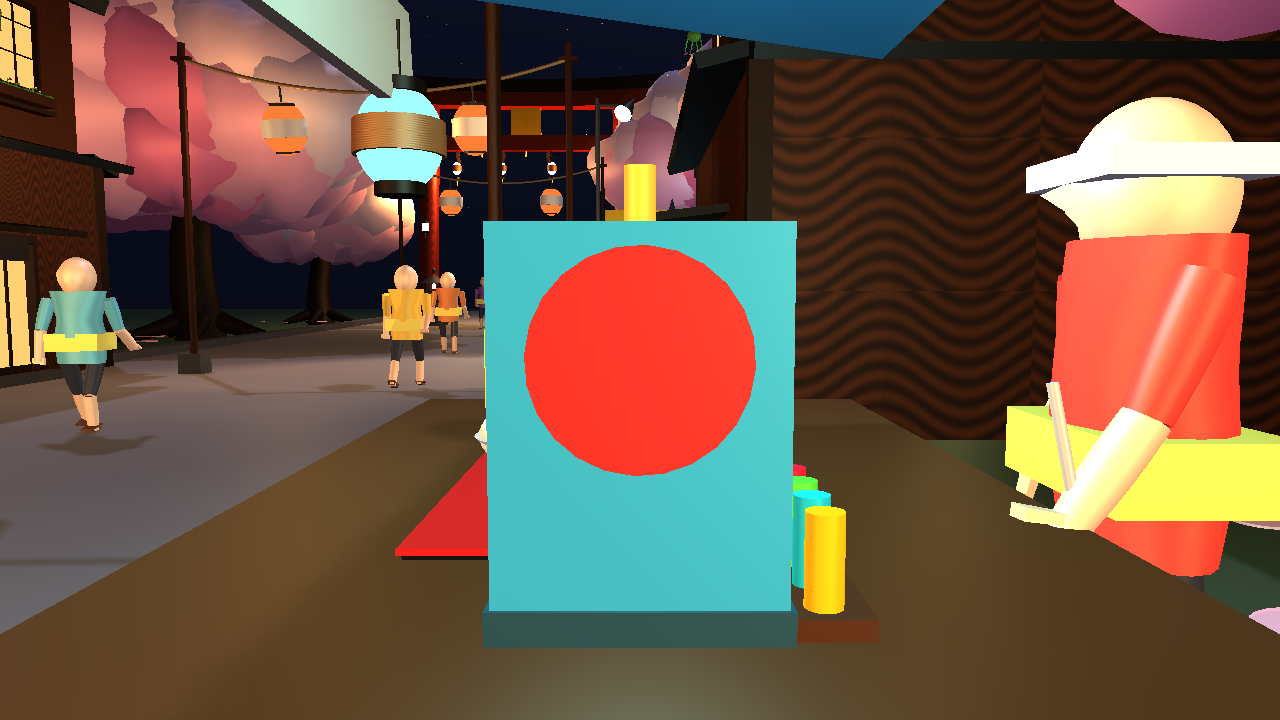
\includegraphics[width=\textwidth]{figures/ss_07_kakigori_stall.png}%
  }{\fbox{ss\_07}}
  \caption{Kakigori Shaved Ice Dessert Stall}
  \label{fig:kakigori_stall}
\end{subfigure}
\caption{Festival food stall animations and complex moving assemblies.}
\label{fig:stalls_figures}
\end{figure}

\section{System 4: Vanishing Box 5-Phase Illusion Sequence}
The vanishing box trick (\texttt{src/Objects.h: lines 4246--4355}) operates via a state machine tracked by \texttt{stateTimer}:
\begin{itemize}
    \item \textbf{Phase 1 (0.0s -- 2.0s) --- Levitation:} Golden box hovers upward from the table ($\Delta y = 0.35\,\text{m}$) using a smooth cubic ease-in-out curve.
    \item \textbf{Phase 2 (2.0s -- 3.2s) --- Rapid Spin:} Box accelerates spin about the vertical axis ($\omega_y = 720^\circ/\text{s}$).
    \item \textbf{Phase 3 (3.2s -- 4.2s) --- Vanishing Scale:} Non-uniform scale collapses to zero:
    \begin{equation}
    \mathbf{S}(t) = \mathbf{S}_0 \cdot \left( 1.0 - \tau^3 \right), \quad \tau = \frac{t - 3.2}{1.0}
    \end{equation}
    \item \textbf{Phase 4 (4.2s -- 6.0s) --- Absence:} Box is completely invisible (\texttt{visible = false}); the magician gestures to the empty table.
    \item \textbf{Phase 5 ($> 6.0\text{s}$) --- Replay:} Cycle resets or can be triggered at any time via Key \textbf{M}.
\end{itemize}

\section{System 5: Hierarchical Pedestrian Crowd Walking}
The pedestrian crowd figures walking down the street possess a 10-bone hierarchical character rig:
\begin{itemize}
    \item \textbf{Linear Translation:} The root node advances down the street at $v_{\text{walk}} = 1.15\,\text{m/s}$. When $z < -30.0\,\text{m}$, the walker wraps around to $+28.0\,\text{m}$.
    \item \textbf{Counter-Phase Hip Swings:} Left and right hip joints swing out of phase: $\theta_{\text{hip, L}} = \theta_{\text{leg}} \sin(\omega t)$, $\theta_{\text{hip, R}} = -\theta_{\text{leg}} \sin(\omega t)$ ($\theta_{\text{leg}} = 26.0^\circ$).
    \item \textbf{Realistic Knee Flexion:} Knees only bend backwards during the swing phase:
    \begin{equation}
    \theta_{\text{knee}} = \max\left( 0.0, -\theta_{\text{hip}} \cdot 0.85 \right)
    \end{equation}
    \item \textbf{Counter-Phase Arm Swings:} Left arm swings opposite to left leg to balance angular momentum ($\theta_{\text{arm}} = 18.0^\circ$).
    \item \textbf{Torso Bobbing:} Vertical bobbing simulates the gait cycle: $y = y_0 + 0.04 \cdot |\sin(\omega t)|$.
\end{itemize}

\begin{figure}[H]
\centering
\begin{subfigure}[b]{0.48\textwidth}
  \centering
  \IfFileExists{figures/ss_19_crowd_walkers.png}{%
    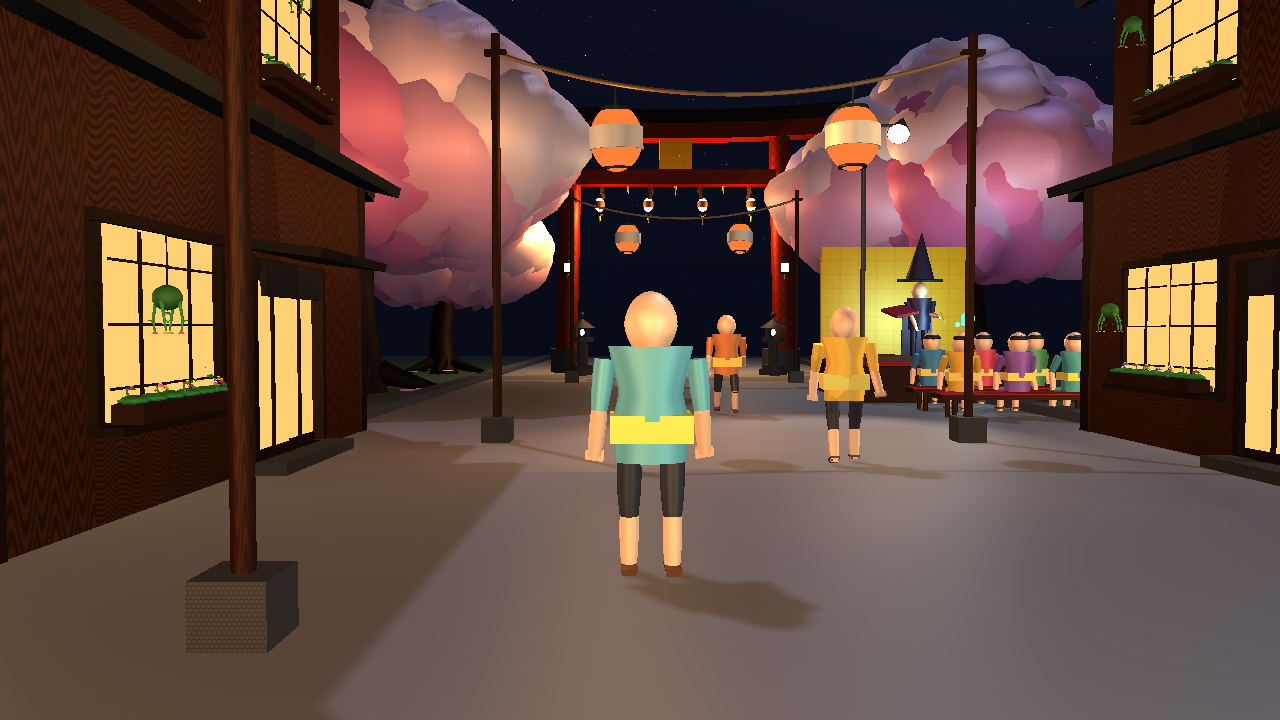
\includegraphics[width=\textwidth]{figures/ss_19_crowd_walkers.png}%
  }{\fbox{ss\_19}}
  \caption{Pedestrian Crowd Walking Limb Cycles}
  \label{fig:crowd_walkers}
\end{subfigure}\hfill
\begin{subfigure}[b]{0.48\textwidth}
  \centering
  \IfFileExists{figures/ss_20_fireworks_burst.png}{%
    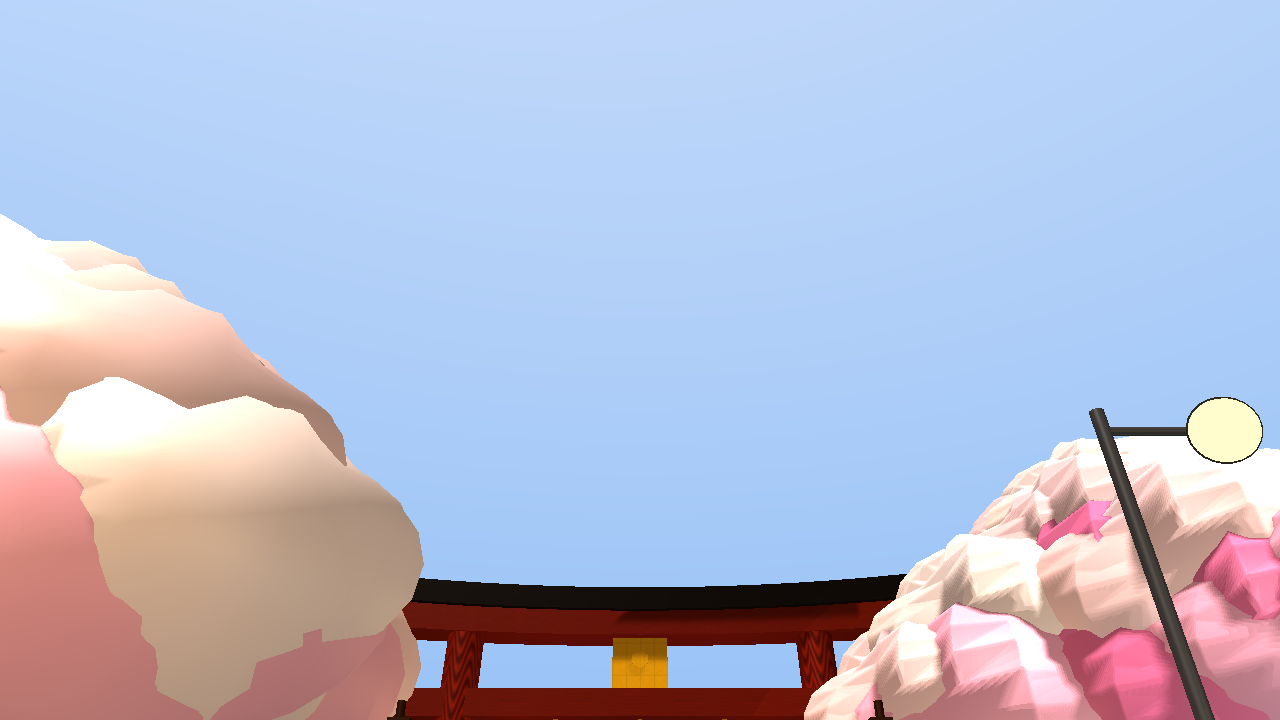
\includegraphics[width=\textwidth]{figures/ss_20_fireworks_burst.png}%
  }{\fbox{ss\_20}}
  \caption{Apex Fireworks Sky Burst Particle Flash}
  \label{fig:fireworks_burst}
\end{subfigure}
\caption{Dynamic crowd pedestrians and sky particle fireworks.}
\label{fig:crowd_fireworks_figures}
\end{figure}

\section{System 6: Interactive Sliding Shoji Doors and Windows}
\subsection{Proximity Detection and Smoothstep Sliding}
When the camera approaches within 5.0 meters of any Machiya building entrance, pressing \textbf{H} toggles the front Shoji entrance door, while pressing \textbf{G} toggles the sliding windows. The sliding progress $\tau \in [0, 1]$ transitions smoothly across $T = 0.65\,\text{s}$ using cubic Hermite interpolation:
\begin{equation}
\operatorname{smoothstep}(\tau) = 3\tau^2 - 2\tau^3, \quad x(t) = x_{\text{closed}} + \Delta x_{\text{max}} \cdot \operatorname{smoothstep}(\tau)
\end{equation}
where max doorway travel $\Delta x_{\text{max}} = 1.45\,\text{m}$ and window travel is $0.90\,\text{m}$.

\begin{figure}[H]
\centering
\begin{subfigure}[b]{0.48\textwidth}
  \centering
  \IfFileExists{figures/ss_08_machiya_exterior.png}{%
    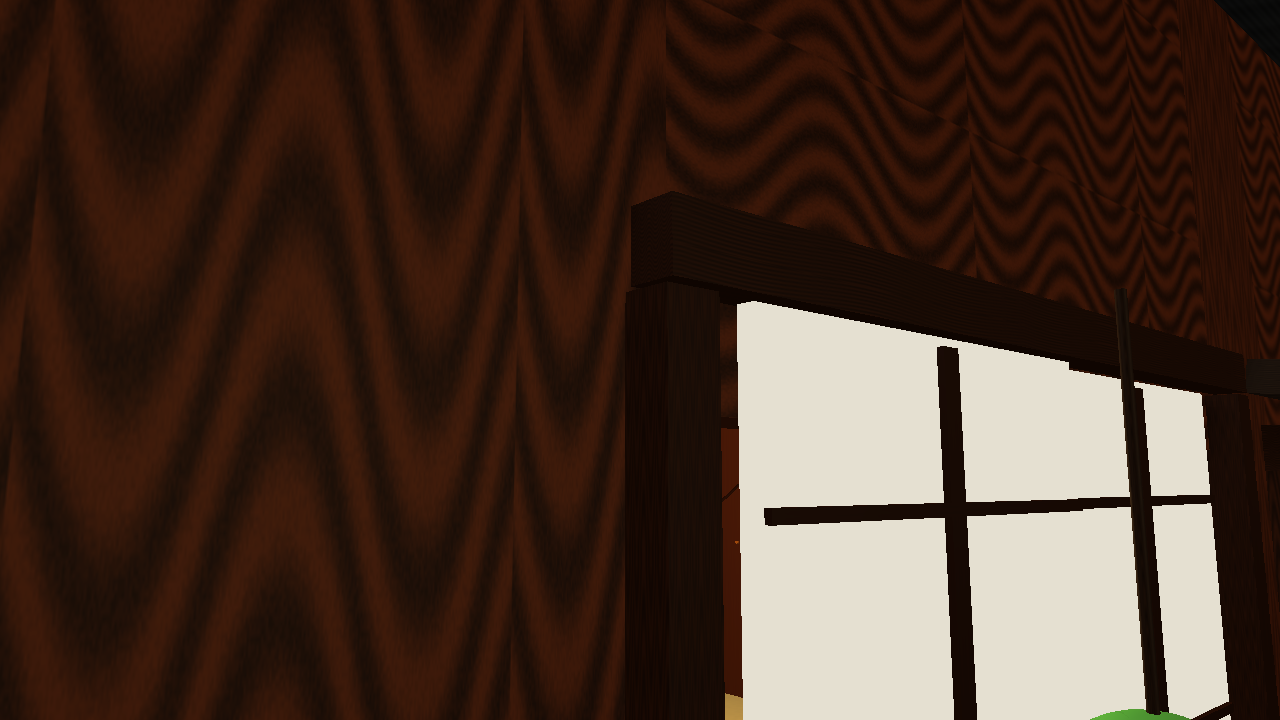
\includegraphics[width=\textwidth]{figures/ss_08_machiya_exterior.png}%
  }{\fbox{ss\_08}}
  \caption{Exterior View of Townhouses L1 \& L2}
  \label{fig:machiya_ext}
\end{subfigure}\hfill
\begin{subfigure}[b]{0.48\textwidth}
  \centering
  \IfFileExists{figures/ss_09_machiya_interior_shoji.png}{%
    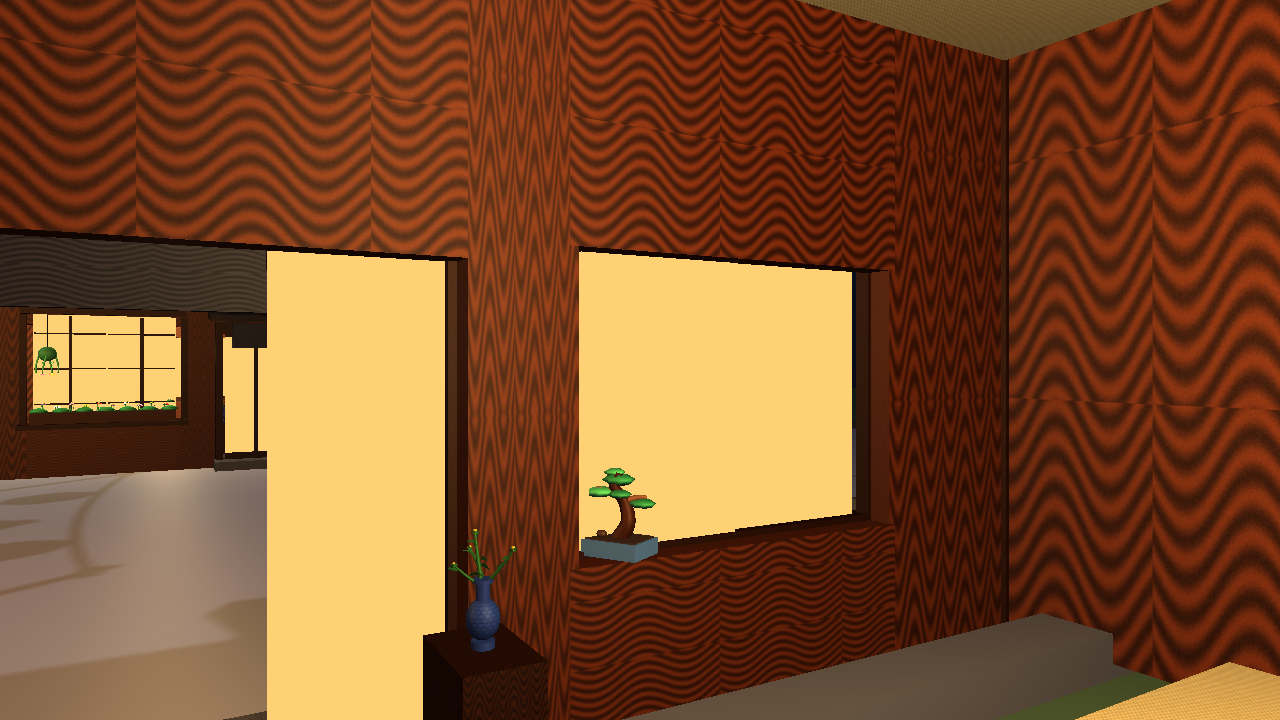
\includegraphics[width=\textwidth]{figures/ss_09_machiya_interior_shoji.png}%
  }{\fbox{ss\_09}}
  \caption{Interior View through Open Shoji Door}
  \label{fig:machiya_int}
\end{subfigure}
\caption{Traditional Machiya townhouses and interactive sliding Shoji doors.}
\label{fig:machiya_figures}
\end{figure}

\subsection{Continuous Collision Detection and Doorway Portals}
Pressing the \textbf{B} key toggles between \textbf{Walk Mode} (solid walls and collision active) and \textbf{Noclip Mode} (free flying). In Walk Mode:
\begin{enumerate}
    \item Bounding boxes encase Machiya foundation walls ($X \in [-14.5, -6.5]$, $Z \in [11.5, 20.5]$).
    \item \textbf{Dynamic Doorway Portal:} A passage window is defined at $Z \in [-2.05, +0.25]\,\text{m}$ and $Y \in [0.0, 2.55]\,\text{m}$. If \texttt{isDoorOpen == false}, the door acts as an impenetrable barrier, clamping camera position. When \texttt{isDoorOpen == true}, the portal opens, allowing the player to freely walk from the outdoor street into the interior living room.
    \item \textbf{14-Step Staircase Elevation:} Inside the house, walking onto the staircase footprint smoothly interpolates player elevation $Y$ from ground floor level ($0.2\,\text{m}$) to the second floor deck ($4.3\,\text{m}$).
\end{enumerate}

\section{Falling Sakura Petals and Fireworks Particle Physics}
\begin{itemize}
    \item \textbf{Cherry Blossom Petal Drift (\texttt{src/Objects.h: lines 2720--2770}):} Twelve animated petal nodes execute downward gravitational descent coupled with lateral sinusoidal wind swaying:
    \begin{equation}
    x(t) = x_0 + A_{\text{wind}} \sin(\omega_w t + \phi), \quad y(t) = y_0 - v_{\text{fall}} t \pmod{H_{\text{canopy}}}
    \end{equation}
    \item \textbf{Fireworks Particle Rockets (\texttt{src/Objects.h: lines 4917--5110}):} Pressing \textbf{F} launches an upward rocket with velocity $v_y = 28\,\text{m/s}$. Upon reaching apex altitude ($y \approx 45\,\text{m}$), the rocket explodes into a spherical cloud of expanding colored spark particles affected by air drag and gravity. Point Light 5 flashes at the burst center, casting dramatic transient illumination across the town.
\end{itemize}

\begin{figure}[H]
\centering
\begin{subfigure}[b]{0.48\textwidth}
  \centering
  \IfFileExists{figures/ss_03_torii_gate.png}{%
    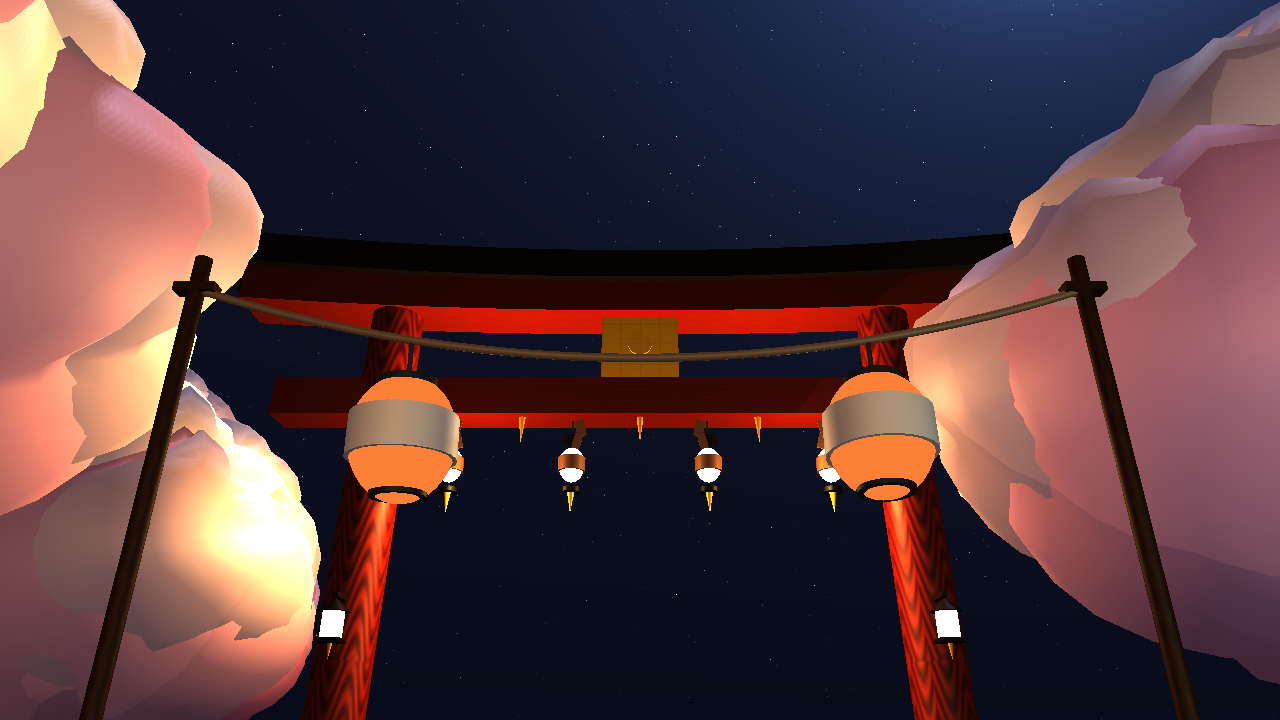
\includegraphics[width=\textwidth]{figures/ss_03_torii_gate.png}%
  }{\fbox{ss\_03}}
  \caption{Grand Torii Shrine Gate with Lanterns}
  \label{fig:torii_gate}
\end{subfigure}\hfill
\begin{subfigure}[b]{0.48\textwidth}
  \centering
  \IfFileExists{figures/ss_10_sakura_tree_petals.png}{%
    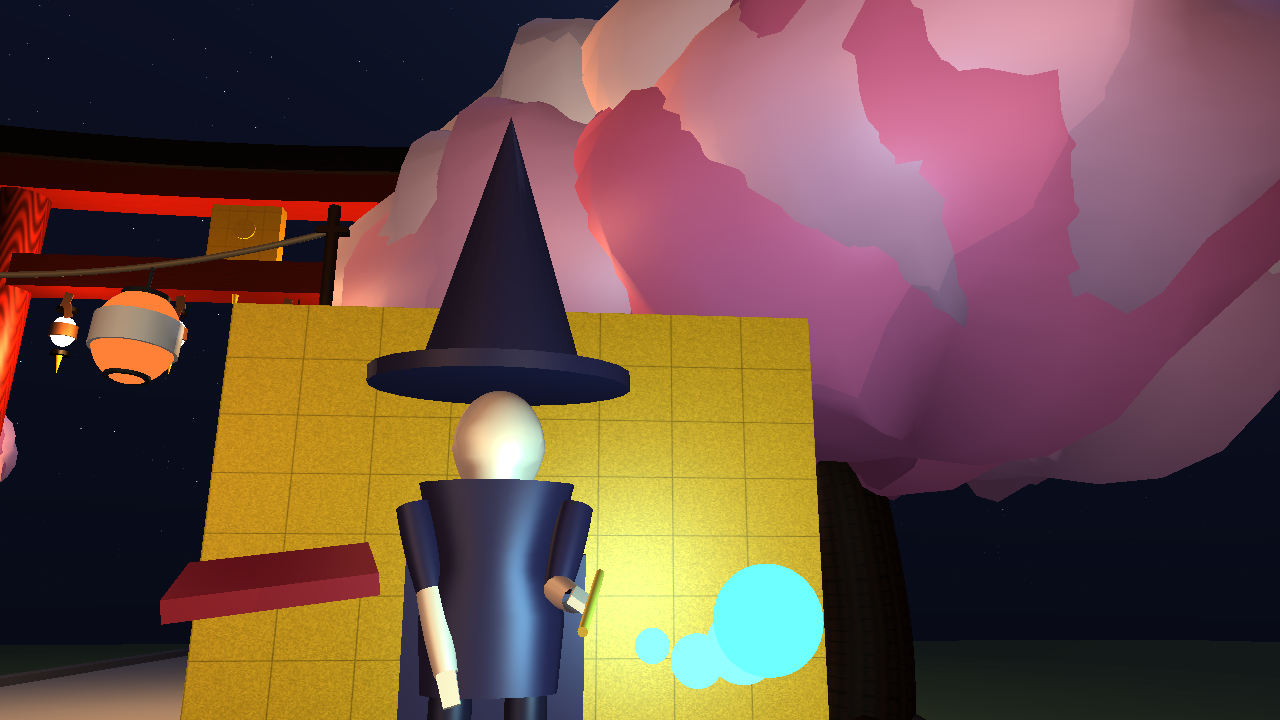
\includegraphics[width=\textwidth]{figures/ss_10_sakura_tree_petals.png}%
  }{\fbox{ss\_10}}
  \caption{Sakura Blossom Tree with Falling Petals}
  \label{fig:sakura_tree}
\end{subfigure}
\caption{Cultural landmarks: Grand Torii shrine gate and cherry blossom tree.}
\label{fig:cultural_landmarks}
\end{figure}
